
\section{Conclusion and Future Steps}



\begin{frame}
	\frametitle{Next: Richer content models}
	\begin{itemize}
		\item Look at anaphors explicitly with local context (e.g. ``plug in'')
		\item More data
		\item Link structure in Wikipedia (e.g., redirects)
		\item Lookahead
	\end{itemize}
\end{frame}

\begin{frame}
	\frametitle{Next: Richer interactions}
		\begin{itemize}
			\item Currently users competing against themselves
			\item But how you play depends on opponents
			\item Rollout of strategies?~\cite{tesauro-96}
			\item Better theoretical grounding~\cite{li-08}
			\item More complicated interface
			\item Game theory to estimate policies
			\item More fun
		\end{itemize}
\end{frame}

\begin{frame}
	\frametitle{Next: Linguistic effects}
		\begin{itemize}
			\item Posterior over answers and latent structure
			\item Can we capture interaction with syntax (e.g. tweaking sentence)
			\item Way of validating psycholinguistic theories about surprisal
		\end{itemize}
\end{frame}

\begin{frame}{Simultaneous Translation}
  \centering
  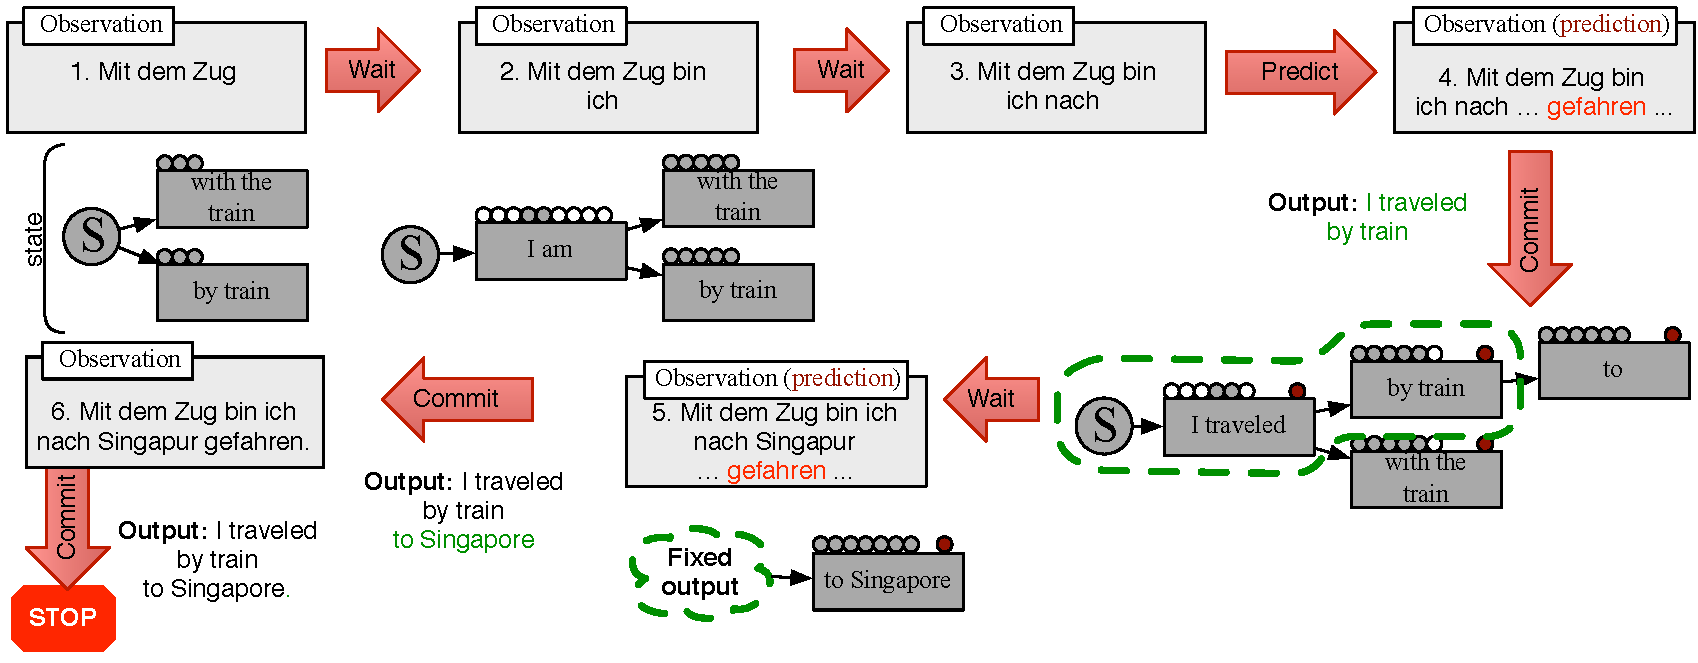
\includegraphics[width=1.0\linewidth]{qb/incremental_translation}
\end{frame}

\begin{frame}

	\frametitle{Recap}

	\begin{itemize}
			\item Fun and useful for users
			\item Improves batch learning
			\item Learning incremental classification by example
	\end{itemize}
\end{frame}
